\RequirePackage{luatex85}


\documentclass{standalone}
\usepackage{tikz} 
%include other needed packages here
\usepackage{tikz-feynman}

% Blue: #0000FF (r,g,b) = (0,0,1) Red: #FF0000 (r,g,b) = (1,0,0) Green: #228B22 (r,g,b) = (0.13, 0.55, 0.13)
\definecolor{cB}{rgb}{0,0,1}
\definecolor{cR}{rgb}{1,0,0}
\definecolor{cG}{rgb}{0.13, 0.55, 0.13}

\tikzfeynmanset{compat=1.0.0}

\tikzset{myblob/.style={
  shape=circle,
  draw=black,
  fill=black,
  minimum size=0.60cm,
  scale=0.40,
  text = black,
  }
}

\tikzset{blobber/.style={
  shape=circle,
  draw=black,
  fill=black,
  minimum size=0.60cm,
  scale=0.10,
  text = black,
  }
}

\tikzset{myblob2/.style={
  shape=circle,
  draw=red,
  fill=red,
  minimum size=0.60cm,
  scale=0.40,
  text = red,
  }
}

\tikzset{myblobG/.style={
  shape=circle,
  draw=cG,
  fill=cG,
  minimum size=0.60cm,
  scale=0.40,
  text = cG,
  }
}

\tikzset{myblobB/.style={
  shape=circle,
  draw=cB,
  fill=cB,
  minimum size=0.60cm,
  scale=0.40,
  text = cB,
  }
}

\usepackage{graphicx}
\usepackage{caption}
\usepackage{subcaption}

\begin{document}

%%%%%%%%%%%%%%%% gg -> X -> YH
\iffalse
    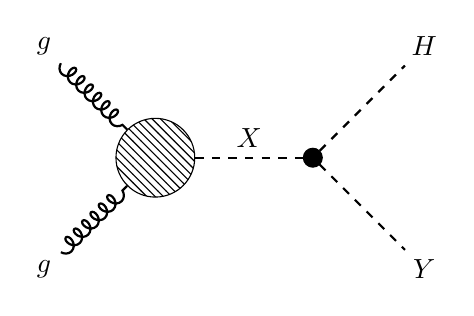
\begin{tikzpicture}[]
      \begin{feynman}[large]
        \vertex [,blob] (m1) {} ;
        \vertex [right =of m1, myblob] (m2)  { };

        \vertex [above left =of m1] (i1) { \( g \)};;
        \vertex [below left =of m1] (i2) { \( g \)};;

        \vertex [above right =of m2] (f1)  { \( H \) };
        \vertex [below right =of m2] (f2)  { \( Y \) };

        \diagram* {
          (i1) -- [gluon] (m1),
          (i2) -- [gluon] (m1),

          (m1) -- [scalar, edge label=\(X\)] (m2),
          
          (m2) -- [scalar,  ] (f1),
          (m2) -- [scalar,  ] (f2),
        };
      \end{feynman}
    \end{tikzpicture}
\fi 
%%%%%%%%%%%%%%%% y_t
\iffalse
    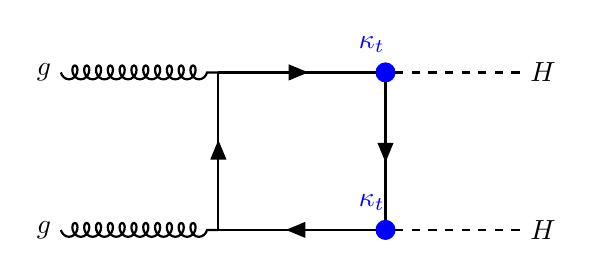
\begin{tikzpicture}[]
      \begin{feynman}[large]
        \vertex [,] (m1)  ;
        \vertex [label=\({ \textcolor{cB}{\kappa_t }}~~~\), myblobB, right =of m1] (m2)  { };
        \vertex [label=\({ \textcolor{cB}{\kappa_t }}~~~\), myblobB, below =of m2] (m3)  { };
        \vertex [, , below =of m1] (m4) ;

        \vertex [left =of m1] (i1) { \( g \)};;
        \vertex [left =of m4] (i2) { \( g \)};;

        \vertex [right = of m2 ] (f1)  { \( H \) };
        \vertex [right = of m3 ] (f2)  { \( H \) };

        
        \diagram* {
          (i1) -- [gluon] (m1),
          (i2) -- [gluon] (m4),

          (m1) -- [fermion] (m2),
          (m2) -- [fermion] (m3),
          (m3) -- [fermion] (m4),
          (m4) -- [fermion] (m1),
          
          (m2) -- [scalar,  ] (f1),
          (m3) -- [scalar,  ] (f2),
        };
      \end{feynman}
    \end{tikzpicture}
\fi 

%%%%%%%%%%%%%%%% c_{g} \lambda_{HHH}
\iffalse
    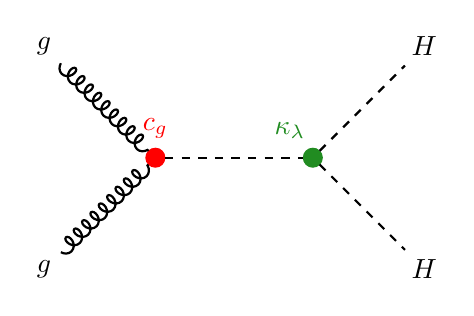
\begin{tikzpicture}[]
      \begin{feynman}[large]
        \vertex [label=\({ \textcolor{cR}{c_{g}} }\), myblob2] (m1)  { };
        \vertex [above left =of m1] (i1){ \( g \)};
        \vertex [below left =of m1] (i2){ \( g \)};
        \vertex [right = of m1, myblobG, label=\({\textcolor{cG}{\kappa_{\lambda}}~~~~~}\) ] (m2)  { };
        \vertex [above right = of m2 ] (f1)  { \( H \) };
        \vertex [below right = of m2 ] (f2)  { \( H \) };

        
        \diagram* {
          (i1) -- [gluon] (m1),
          (i2) -- [gluon] (m1),
          (m2) -- [scalar,  ] (f1),
          (m2) -- [scalar,  ] (f2),
          (m1) -- [scalar,  ] (m2),
        };
      \end{feynman}
    \end{tikzpicture}
\fi 

%%%%%%%%%%%%%%%% c_{2g}
\iffalse
    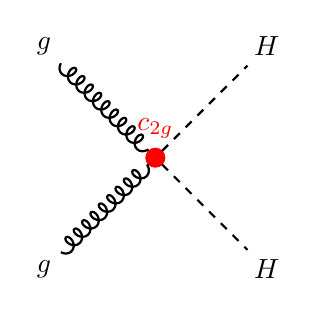
\begin{tikzpicture}[]
      \begin{feynman}[large]
        \vertex [label=\({ \textcolor{cR}{c_{2g}} }\), myblob2] (m1)  { };
        \vertex [above left =of m1] (i1){ \( g \)};
        \vertex [below left =of m1] (i2){ \( g \)};
        \vertex [above right = of m1 ] (f1)  { \( H \) };
        \vertex [below right = of m1 ] (f2)  { \( H \) };

        
        \diagram* {
          (i1) -- [gluon] (m1),
          (i2) -- [gluon] (m1),
          (m1) -- [scalar,  ] (f1),
          (m1) -- [scalar,  ] (f2),
        };
      \end{feynman}
    \end{tikzpicture}
\fi 

%%%%%%%%%%%%%%%% c_2
\iffalse
    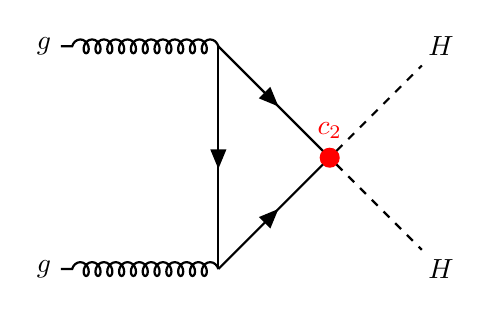
\begin{tikzpicture}[]
      \begin{feynman}[large]
        \vertex [label=\({ \textcolor{cR}{c_2} }\), myblob2] (m1)  { };
        \vertex [above left =of m1] (i1);
        \vertex [below left =of m1] (i2);
        \vertex [left =of i1] (i11) { \( g \)};
        \vertex [left =of i2] (i21) { \( g \)};
        \vertex [above right = of m1 ] (f1)  { \( H \) };
        \vertex [below right = of m1 ] (f2)  { \( H \) };

        
        \diagram* {
          (i1) -- [gluon] (i11),
          (i2) -- [gluon] (i21),
          (i1) -- [fermion] (i2),
          (i1) -- [fermion] (m1),
          (i2) -- [fermion] (m1),
          (m1) -- [scalar,  ] (f1),
          (m1) -- [scalar,  ] (f2),
        };
      \end{feynman}
    \end{tikzpicture}
\fi 

%%%%%%%%%%%%%%%% y_t \lambda_{HHH}
%%\iffalse
    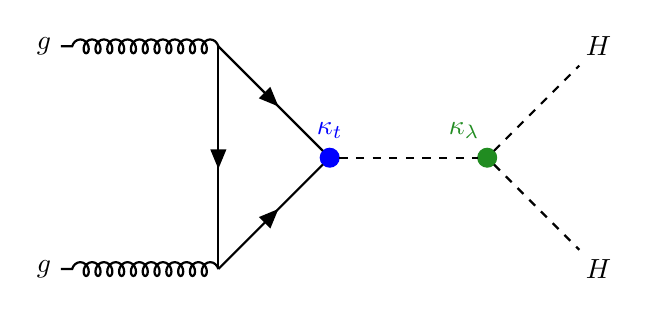
\begin{tikzpicture}[]
      \begin{feynman}[large]
        \vertex [label=\({ \textcolor{cB}{\kappa_{t}} }\), myblobB] (m1)  { };
        \vertex [above left =of m1] (i1);
        \vertex [below left =of m1] (i2);
        \vertex [left =of i1] (i11) { \( g \)};
        \vertex [left =of i2] (i21) { \( g \)};
        \vertex [right = of m1, myblobG, label=\({\textcolor{cG}{\kappa_{\lambda}~~~~~}}\) ] (m2)  { };
        \vertex [above right = of m2 ] (f1)  { \( H \) };
        \vertex [below right = of m2 ] (f2)  { \( H \) };

        
        \diagram* {
          (i1) -- [gluon] (i11),
          (i2) -- [gluon] (i21),
          (i1) -- [fermion] (i2),
          (i1) -- [fermion] (m1),
          (i2) -- [fermion] (m1),
          (m1) -- [scalar,  ] (m2),
          (m2) -- [scalar,  ] (f1),
          (m2) -- [scalar,  ] (f2),
        };
      \end{feynman}
    \end{tikzpicture}
%\fi 

%%%%%%%%%%%%%%%% OLD

\end{document}
